\section{Experimentos y análisis de resultados}
	
	\subsection{Procedimiento de desarrollo de la práctica}
	
	\paragraph{}Para realizar la práctica, se ha optado por implementar las heurísticas propuestas en el lenguaje de programación \textsc{Java}. El ejecutable que se entrega junto a este documento ha sido compilado bajo \textsc{ Apache NetBeansIDE 12.0}.
	
	\subsubsection{Equipo de pruebas}
	
	\paragraph{}Los resultados de las heurísticas han sido obtenidos en el siguiente equipo:
	
		\begin{itemize}
			
			\item Host:
			\item S.O:
			\item Kernel:
			\item CPU:
			\item GPU:
			\item GPU:
			\item Memoria RAM :
			
		\end{itemize}

	\subsubsection{Manual de usuario}
	
		\paragraph{}Para ejecutar el software asegúrese de que el archivo .jar proporcionado se ubica en el mismo directorio que la carpeta \emph{archivos}. 
		
		\paragraph{}Cuando se muestre la GUI, podrá seleccionar la heurística que desee mediante el botón correspondiente. Una vez empiece la ejecución de una heurística no sera posible seleccionar otra hasta que finalice su ejecución. Los resultados finales se mostrarán en el cuadro de texto, a su vez, se generan los log correspondientes a cada archivo y semilla en la carpeta Log.
	
		\begin{figure}[H]
		
			\centering
			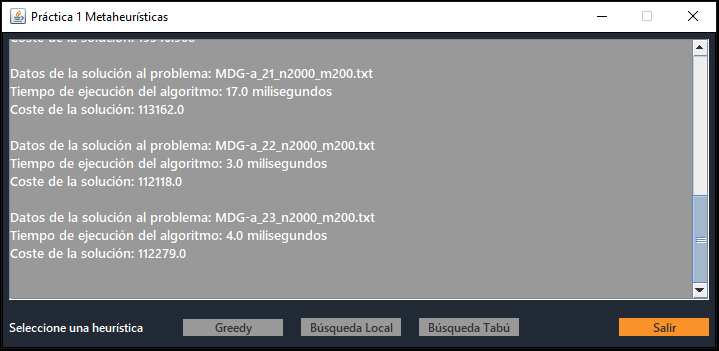
\includegraphics[scale=0.4]{img/GUI}
			\caption{GUI}
		
		\end{figure}
	
	\subsection{Parámetros de los algoritmos}
	
		\subsubsection{Sistema de Colonias de Hormigas}

		\paragraph{}Para regular el comportamiento del Sistema de Colonias de Hormigas, se han definido los siguientes parámetros en el archivo de configuración:
		
		\begin{itemize}
			
			\item Semilla: Número utilizado para la generación de números pseudoaleatorios, valor por defecto : 77356084.
			\item Iteraciones:  Número máximo de iteraciones realizadas por el algoritmo principal, valor por defecto: 10.000.
			\item Número de hormigas: Número de hormigas pertenecientes a cada colonia generada en cada iteración, valor por defecto: 10.
			\item Q0: Probabilidad de no elegir directamente el candidato que mayor coste aporta a la hormiga en la regla de la transición, valor por defecto: 0,95.
			\item Beta: Exponente aplicado al coste de los arcos en las fórmulas de la regla de la transición, valores por defecto: 1 y 2.
			\item Alfa: Exponente aplicado a la feromona de los arcos en las fórmulas de la regla de la transición, valores por defecto: 1 y 2.
			\item Rho: Constante aplicada en la fórmula de la evaporación global de feromona, valor por defecto: 0,1.
			\item Phi: Constante aplicada en la fórmula de la evaporación local de feromona, valor por defecto: 0,1.
			\item Delta: Porcentaje de restricción aplicado sobre la lista de candidatos total de una hormiga, valor por defecto: 0,75.
			
		\end{itemize}
	\subsubsection{Semillas}
	
	\paragraph{}Para la generación de números pseudoaleatorios se utiliza una semilla previamente definida en el archivo de configuración, en este caso es 77356084. Esta semilla se va rotando en las 5 iteraciones de cada archivo.
	
	
	\paragraph{} 77356084 $\rightarrow$ 73560847 $\rightarrow$ 35608477  ...
	
	
	\subsection{Análisis de los resultados}
	
	
